%%%%%%%%%%%%%%%%%%%%%%%%%%%%%%%%%%%%%%%%%%%%%%%%%%%%%%%%%%%%%%%%%%%%
%% I, the copyright holder of this work, release this work into the
%% public domain. This applies worldwide. In some countries this may
%% not be legally possible; if so: I grant anyone the right to use
%% this work for any purpose, without any conditions, unless such
%% conditions are required by law.
%%%%%%%%%%%%%%%%%%%%%%%%%%%%%%%%%%%%%%%%%%%%%%%%%%%%%%%%%%%%%%%%%%%%

\documentclass[
  printed, %% This option enables the default options for the
           %% printed version of a document. Replace with `digital`
           %% to enable the default options for the digital version
           %% of a document.
  table,   %% Causes the coloring of tables. Replace with `notable`
           %% to restore plain tables.
  lof,     %% Prints the List of Figures. Replace with `nolof` to
           %% hide the List of Figures.
  lot,     %% Prints the List of Tables. Replace with `nolot` to
           %% hide the List of Tables.
  %% More options are listed in the user guide at
  %% <http://mirrors.ctan.org/macros/latex/contrib/fithesis/guide/mu/fi.pdf>.
]{fithesis3}

%% The following section sets up the locales used in the thesis.
\usepackage[
  main=slovak, %% By using `czech` or `slovak` as the main locale
               %% instead of `english`, you can typeset the thesis
               %% in either Czech or Slovak, respectively.
  slovak, english %% The additional keys allow
]{babel}          %% foreign texts to be typeset as follows:
				  %%  \begin{otherlanguage}{english}  ... \end{otherlanguage}

\usepackage{paratype}

%% The following section sets up the metadata of the thesis.
\thesissetup{
    date          = \the\year/\the\month/\the\day,
    university    = mu,
    faculty       = fi,
    type          = mgr,
    author        = Matej Majdiš,
    gender        = m,
    advisor       = doc. RNDr. Vlastislav Dohnal\, Ph.D.
    title         = {Rozpoznanie užívateľa na základe informácií o HTTP komunikácií},
    TeXtitle      = {Rozpoznanie užívateľa na základe informácií o HTTP komunikácií},
    keywords      = {keyword1, keyword2, ...},
    TeXkeywords   = {keyword1, keyword2, \ldots},
}

\thesislong{abstract}{
	TODO

}

\thesislong{thanks}{
	TODO
}

%% The following section sets up the bibliography.
\usepackage{csquotes}
\usepackage[              %% When typesetting the bibliography, the
  backend=biber,          %% `numeric` style will be used for the
  style=numeric,          %% entries and the `numeric-comp` style
  citestyle=numeric-comp, %% for the references to the entries. The
  sorting=none,           %% entries will be sorted in cite order.
  sortlocale=auto         %% For more unformation about the available
]{biblatex}               %% `style`s and `citestyles`, see:
%% <http://mirrors.ctan.org/macros/latex/contrib/biblatex/doc/biblatex.pdf>.
\addbibresource{example.bib} %% The bibliograpic database within
                          %% the file `example.bib` will be used.
                          
\usepackage{makeidx}      %% The `makeidx` package contains
\makeindex                %% helper commands for index typesetting.

%% These additional packages are used within the document:
\usepackage{paralist}
\usepackage{amsmath}
\usepackage{amsthm}
\usepackage{amsfonts}
\usepackage{url}
\usepackage{menukeys}
\usepackage{float}
\usepackage[plainpages=false, pdfpagelabels]{hyperref}

\begin{document}

\chapter{Úvod}
Problematika jednoznačnej identifikácie používateľa je dnes veľmi
dôležitou a riešenou témou. Jedným z hlavných dôvodov je fakt, že väčšina
dnešných existujúcich, prípadne novo vznikajúcich systémov a aplikácií je
nejakým spôsobom zapojená do Internetu. Zároveň zaznamenávame nárast
aplikácií, ktoré poskytujú užívateľom webové rozhranie a ústup takzvaných
desktopových aplikácií.

\begin{figure}[h]
  \centering
    
\includegraphics[width=.80\textwidth]{images/web-vs-desktop.png}
  \caption{Vizualizácia pomeru počtu užívateľov webových a desktopových
  aplikácií v čase, zdroj: vlastné spracovanie}
  \label{fig:web-vs-desktop}
\end{figure}

	Z tohto vyplýva potreba rozoznania a identifikácie používateľov, ktorý s
danou aplikáciou interagujú. Existuje niekoľko rôznych prístupov k 
identifikácií, od mapovania IP adries sieťovej vrstvy až po aplikačnú správu
užívateľských účtov. Podrobne sa nimi zaoberá kapitola \ref{ch:existing}.
Cieľom tejto práce je vytvoriť unikátny identifikátor na základe informácií
dostupných z \textit{HTTP} protokolu. Pred zostavením samotného algoritmu je
preto dôležité popísať niektoré kľúčové oblasti a postupy.

Nasledujúce kapitoly sa preto budú stručne zaoberať fungovaním aplikácií typu
klient-server, modelom sieťových vrstiev či útokmi typu \textit{Denial of
Service}. Ďalej v práci popíšem spomínané existujúce prístupy a vlastný návrh
algoritmu identifikácie užívateľa. 

\section{Aplikácie typu Klient-Server}
	S pokračujúcim vývojom nových technológií sa Web stáva stále väčšou
súčasťou našich životov. Web taktiež už nie je limitovaný prehliadaním na
počítačoch. Musí sa prispôsobovať rôznym novým technológiám, ako sú napríklad
mobilné, či iné zriadenia. Najčastejšie používaným modelom komunikácie pre
architektúru webových aplikácií je tzv. Klient-Server model. Základnou
myšlienkou tohto modelu je zaslanie požiadavku (\textit{requestu}) klientom na
server, ktorý vystupuje ako poskytovateľ služby.

\begin{figure}[h]
  \centering
    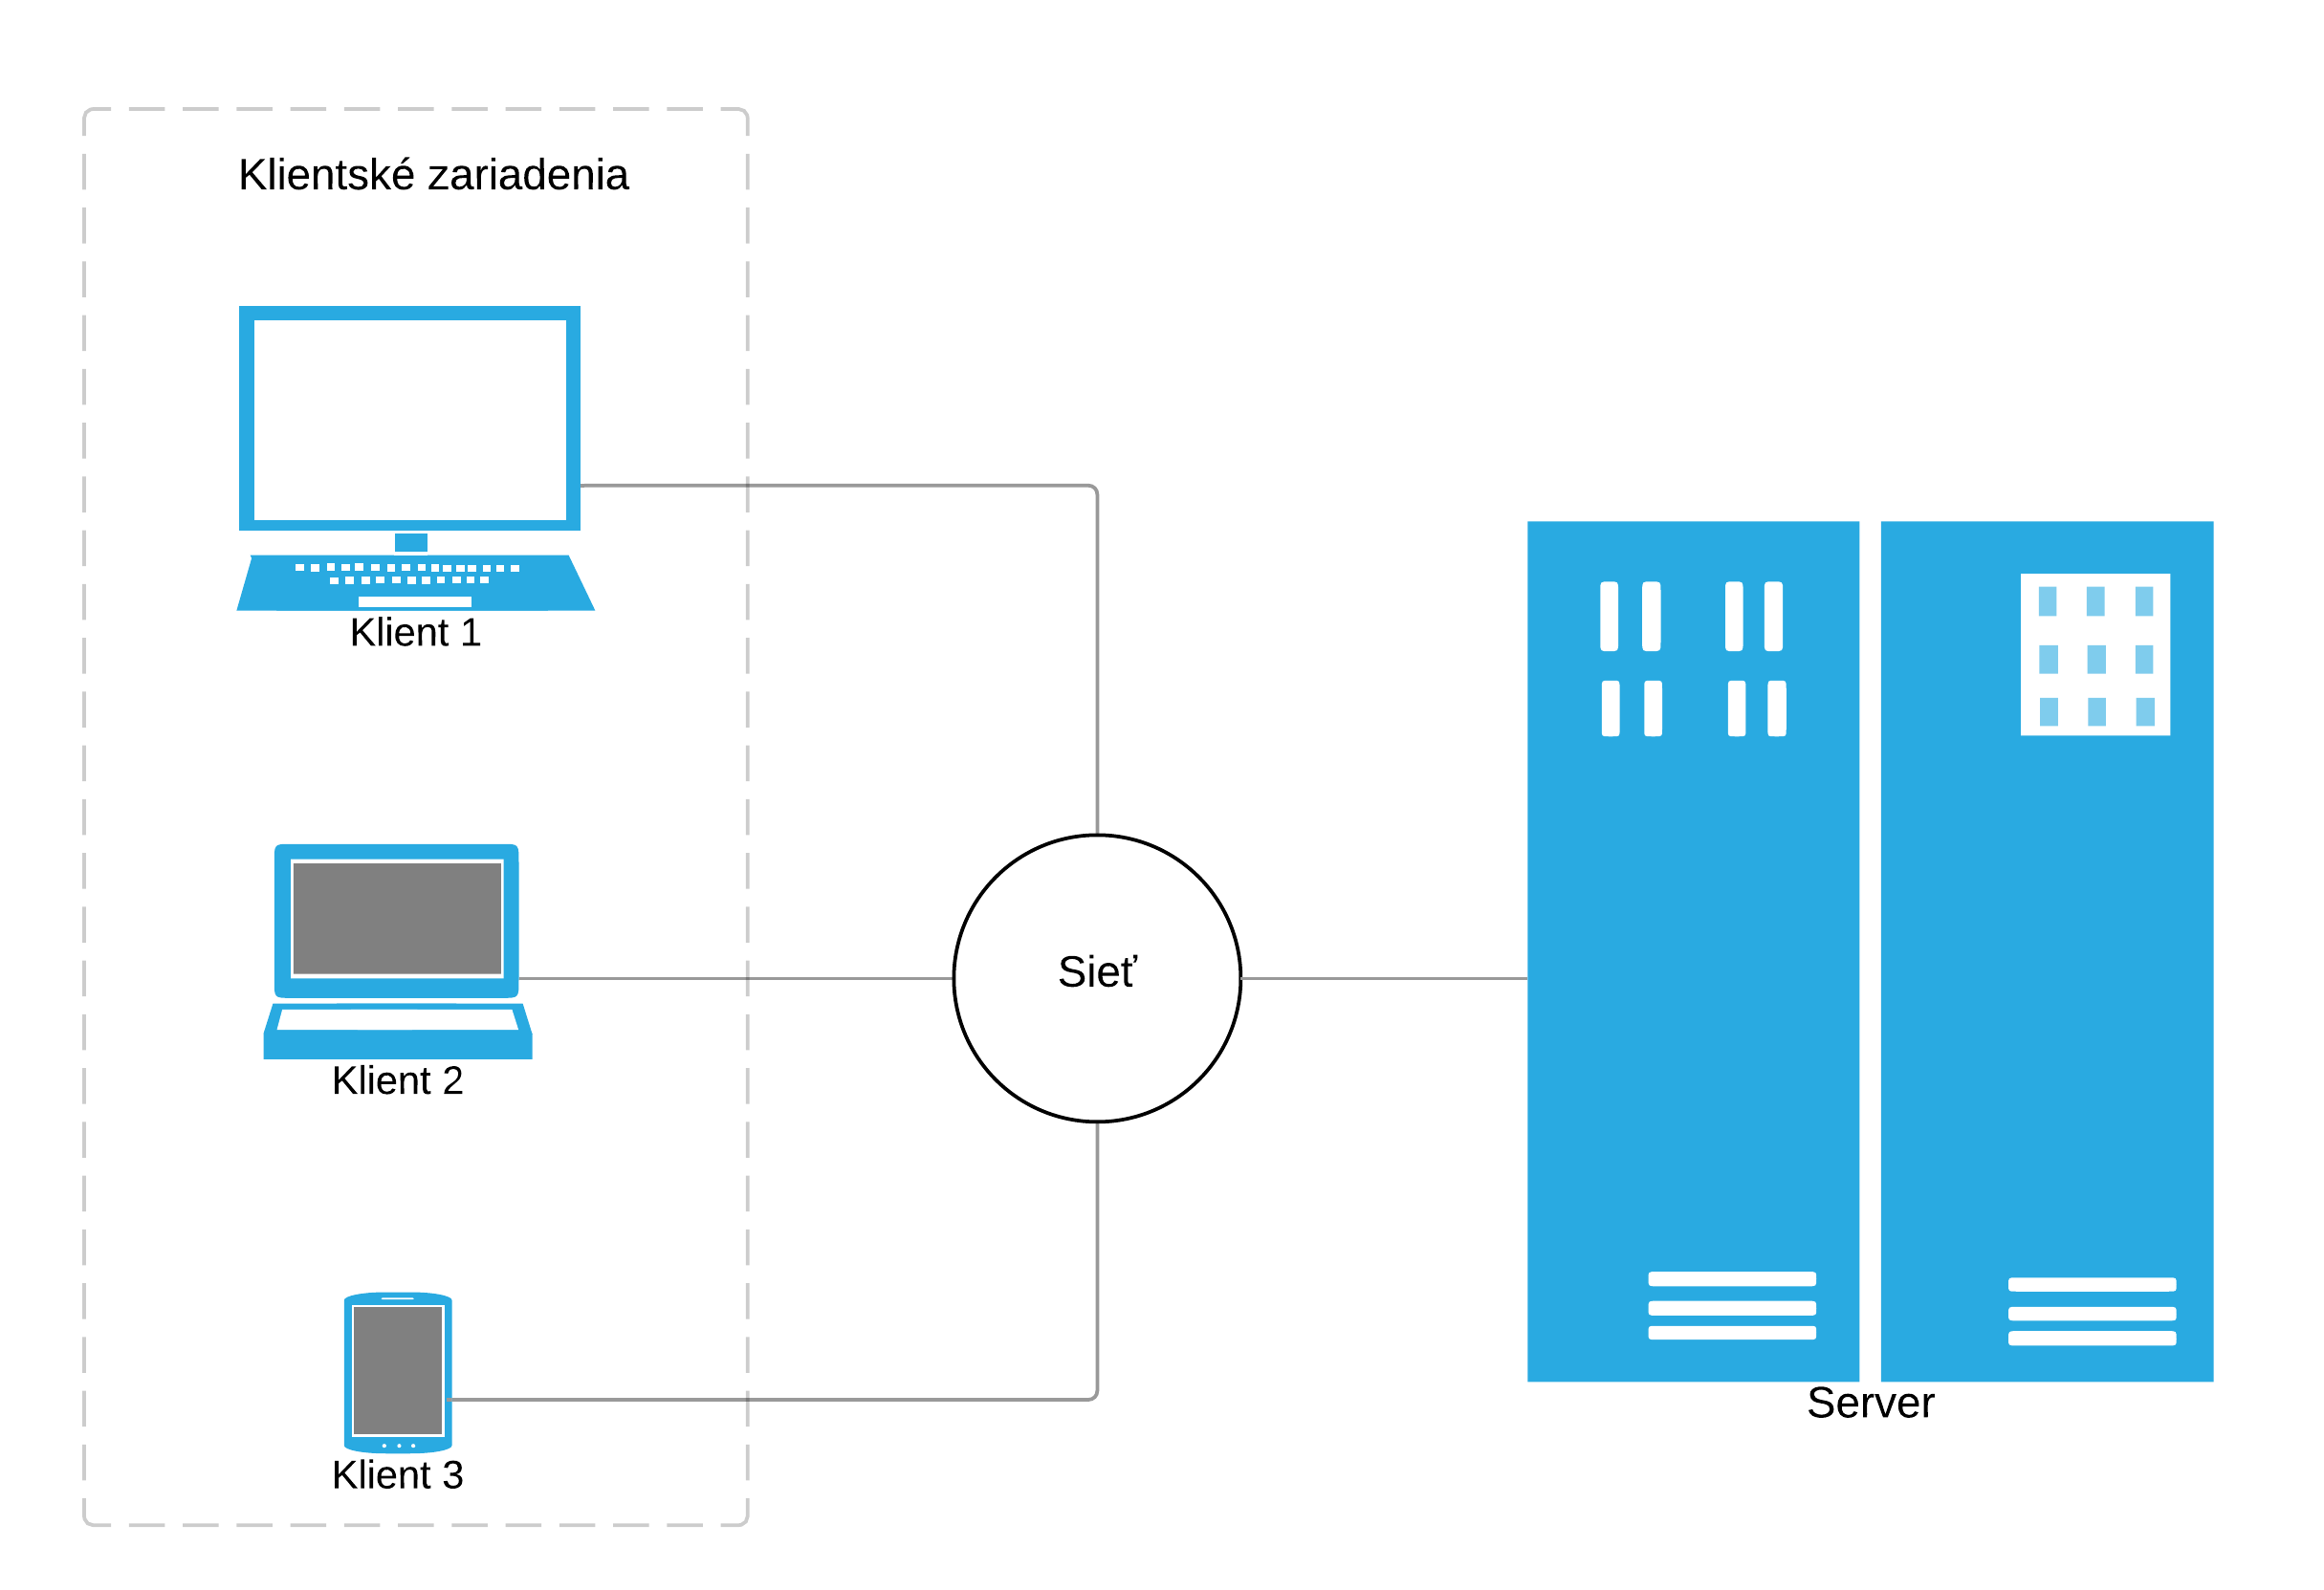
\includegraphics[width=.99\textwidth]{images/C-S-basic.png}
  \caption{Schéma znázorňuje základnú architektúru modelu Klient-Server, zdroj:
  vlastné spracovanie}
  \label{fig:cs-basic}
\end{figure}

\subsection{Klient-Server model}
Pretože Klient-Server model je používaný rôznymi typmi aplikácií bolo nutné
použiť štandardizované protokoly, na základe ktorý ch bude možné komunikovať.
Základné používané protokoly sú: \textit{FTP (File Transfer Protocol)},
\textit{Simple Mail Transfer Protocol (SMTP)} a \textit{Hypertext Transfer
Protocol (HTTP)}. Bližšie sieťové vrstvy a jednotlivé protokoly popisuje
kapitola \ref{ch:net-layers}.

\subsection{Architektúra}
Architektúra modelu Klient-Server sa vo všeobecnosti typicky skladá z troch 
častí:
\begin{itemize}
	\item Aplikačný server
	\item Databázový server
	\item Zariadenie klienta
\end{itemize}
Zároveň Existujú dva základné typy architektúr: 
\begin{itemize}
	\item 2-stupňová \textit{(2-tier)}
	\item 3-stupňová \textit{(3-tier)}
\end{itemize}

\textit{2-tier} architektúra zahrna len zariadenie klienta a databázový server.
U tohoto typu architektúry je aplikácia spustená na zariadení klienta, ktoré sa
následne pripája priamo na server. Zariadenie tak obsluhuje zároveň
\textit{business} logiku aj zobrazovanie aplikácie. Inak tento typ architektúry
nazývame aj tučný klient(\textit{thick client}).

\begin{figure}[H]
  \centering
    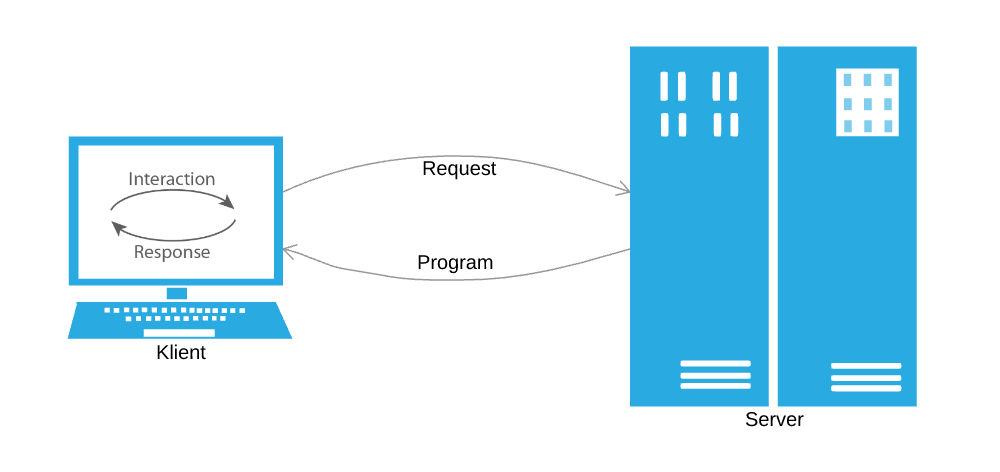
\includegraphics[width=\textwidth]{images/C-S-thick.png}
  \caption{Grafické znázornenie a popis priebehu komunikácie 2-tier architektúry,
  zdroj: vlastné spracovanie}
  \label{fig:cs-thick}
\end{figure}

\textit{3-tier} architektúra, ktorou sa budem zaoberať v tejto práci sa od
\textit{2-tier} líši najmätým, že okrem zariadenia klienta a databázového servera
zahŕňa aj aplikačný server. Tento je následne používaný na obsluhu
\textit{business} logiky aplikácie a komunikáciu s databázou, pričom zariadenie
klienta slúž len na zobrazovanie. Iný názov pre takýto typ architektúry je tenký
klient (\textit{thincient}).

\begin{figure}[H]
  \centering
    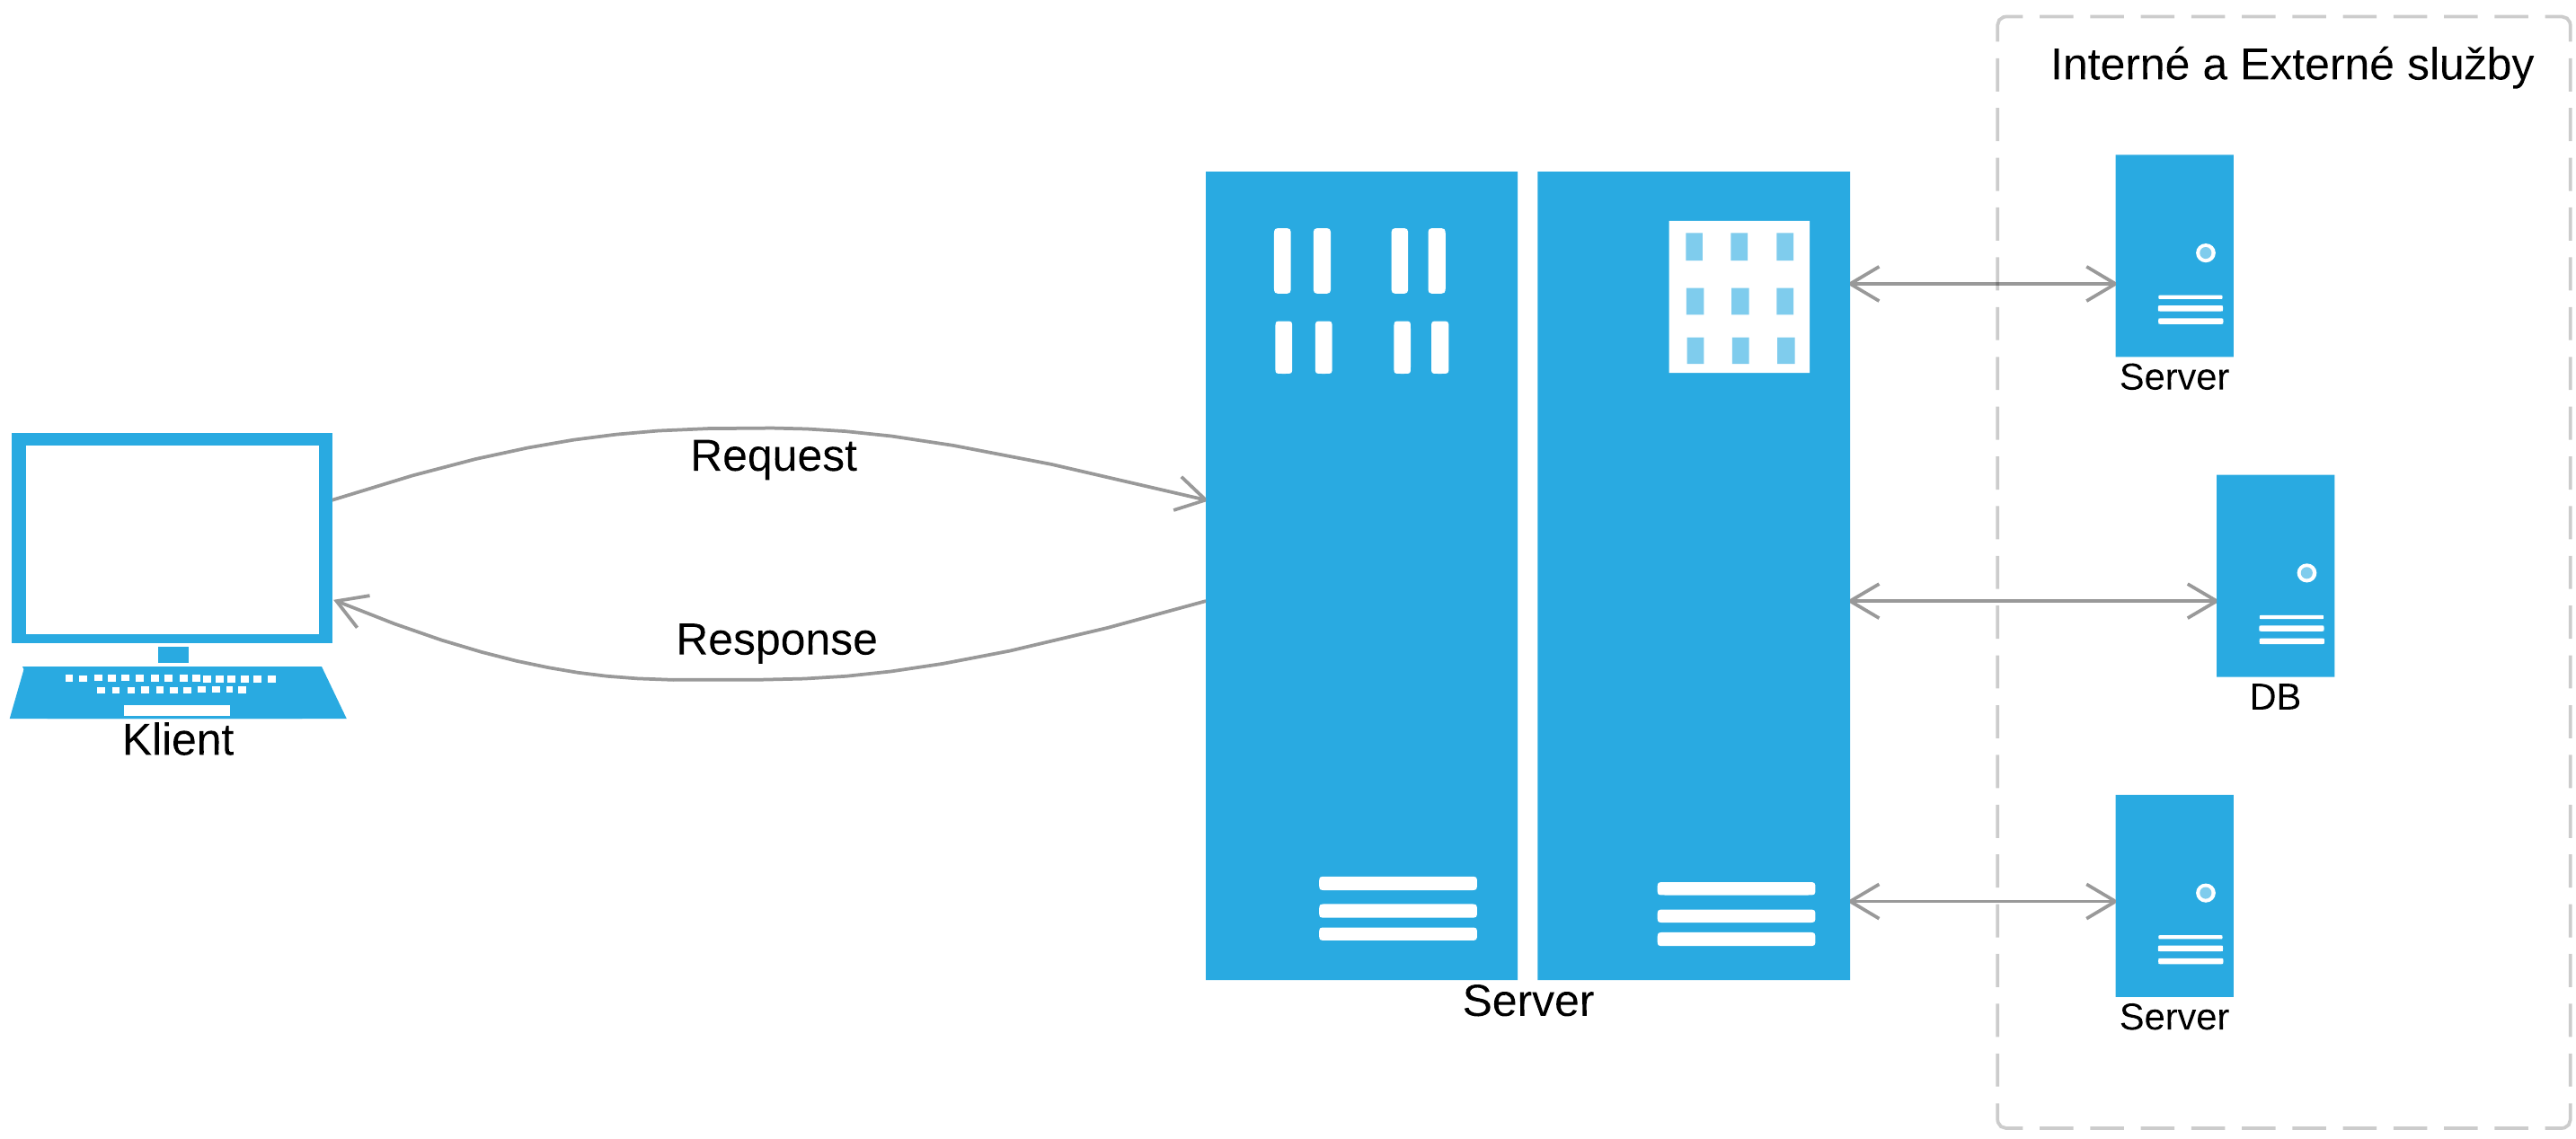
\includegraphics[width=\textwidth]{images/C-S-thin.png}
  \caption{Grafické znázornenie a popis priebehu komunikácie 3-tier architektúry,
  zdroj: vlastné spracovanie}
  \label{fig:cs-thin}
\end{figure}

Nasledujúce kapitoly tejto práce sa budú zaoberať jedným z najdôležitejších
problémov Webových aplikácií, ktorým je identifikácia užívateľa. Najskôr kapitola
\ref{ch:net-layers} analyzuje jednotlivé sieťové vrstvy a protokoly, ktorých
informácie je možné použiť ka následnej identifikácií. Ďalšou časťou je zhrnutie
existujúcich prístupov k rozoznaniu užívateľov v kapitole \ref{ch:existing} a 
popis útokov typu DOS v kapitole \ref{ch:dos}. Najdôležitejšou časťou je však
samozrejme kapitola \ref{ch:footprint}, ktorá popisuje návrh samotného 
algoritmu identifikátoru.

\chapter{Analýza sieťových vrstiev a protokolov}
\label{ch:net-layers}
//TODO - Úvod
\section{Aplikačná vrstva}
\section{Transportná vrstva}
\section{Sieťová vrstva}
\section{Vrstva sieťového rozhrania}

\chapter{Útoky typu \textit{Denial of Service}}
\label{ch:dos}
Jedným z hlavných dôvodov identifikácie užívateľov je prevencia proti útokom. Medzi
najznámejšie z útokov patrí tzv. \textit{Denial of Service}, ďalej len \textit{DoS}.

Vo všeobecnosti je za \textit{DoS} útok považovaná snaha utočníka zabrániť oprávneným
užívateľom v prístupe k informáciám, prípadne službám poskytovateľa. Snahou útočníka
je znefunkčniť pripojenie neustálym narúšaním služby serveru, prípadne sieťovej
infraštruktúry, v dôsledku čoho môže dôjsť k čiastočnej, či úplnej strate
internetového pripojenia hostiteľa. 

\begin{figure}[h]
  \centering
    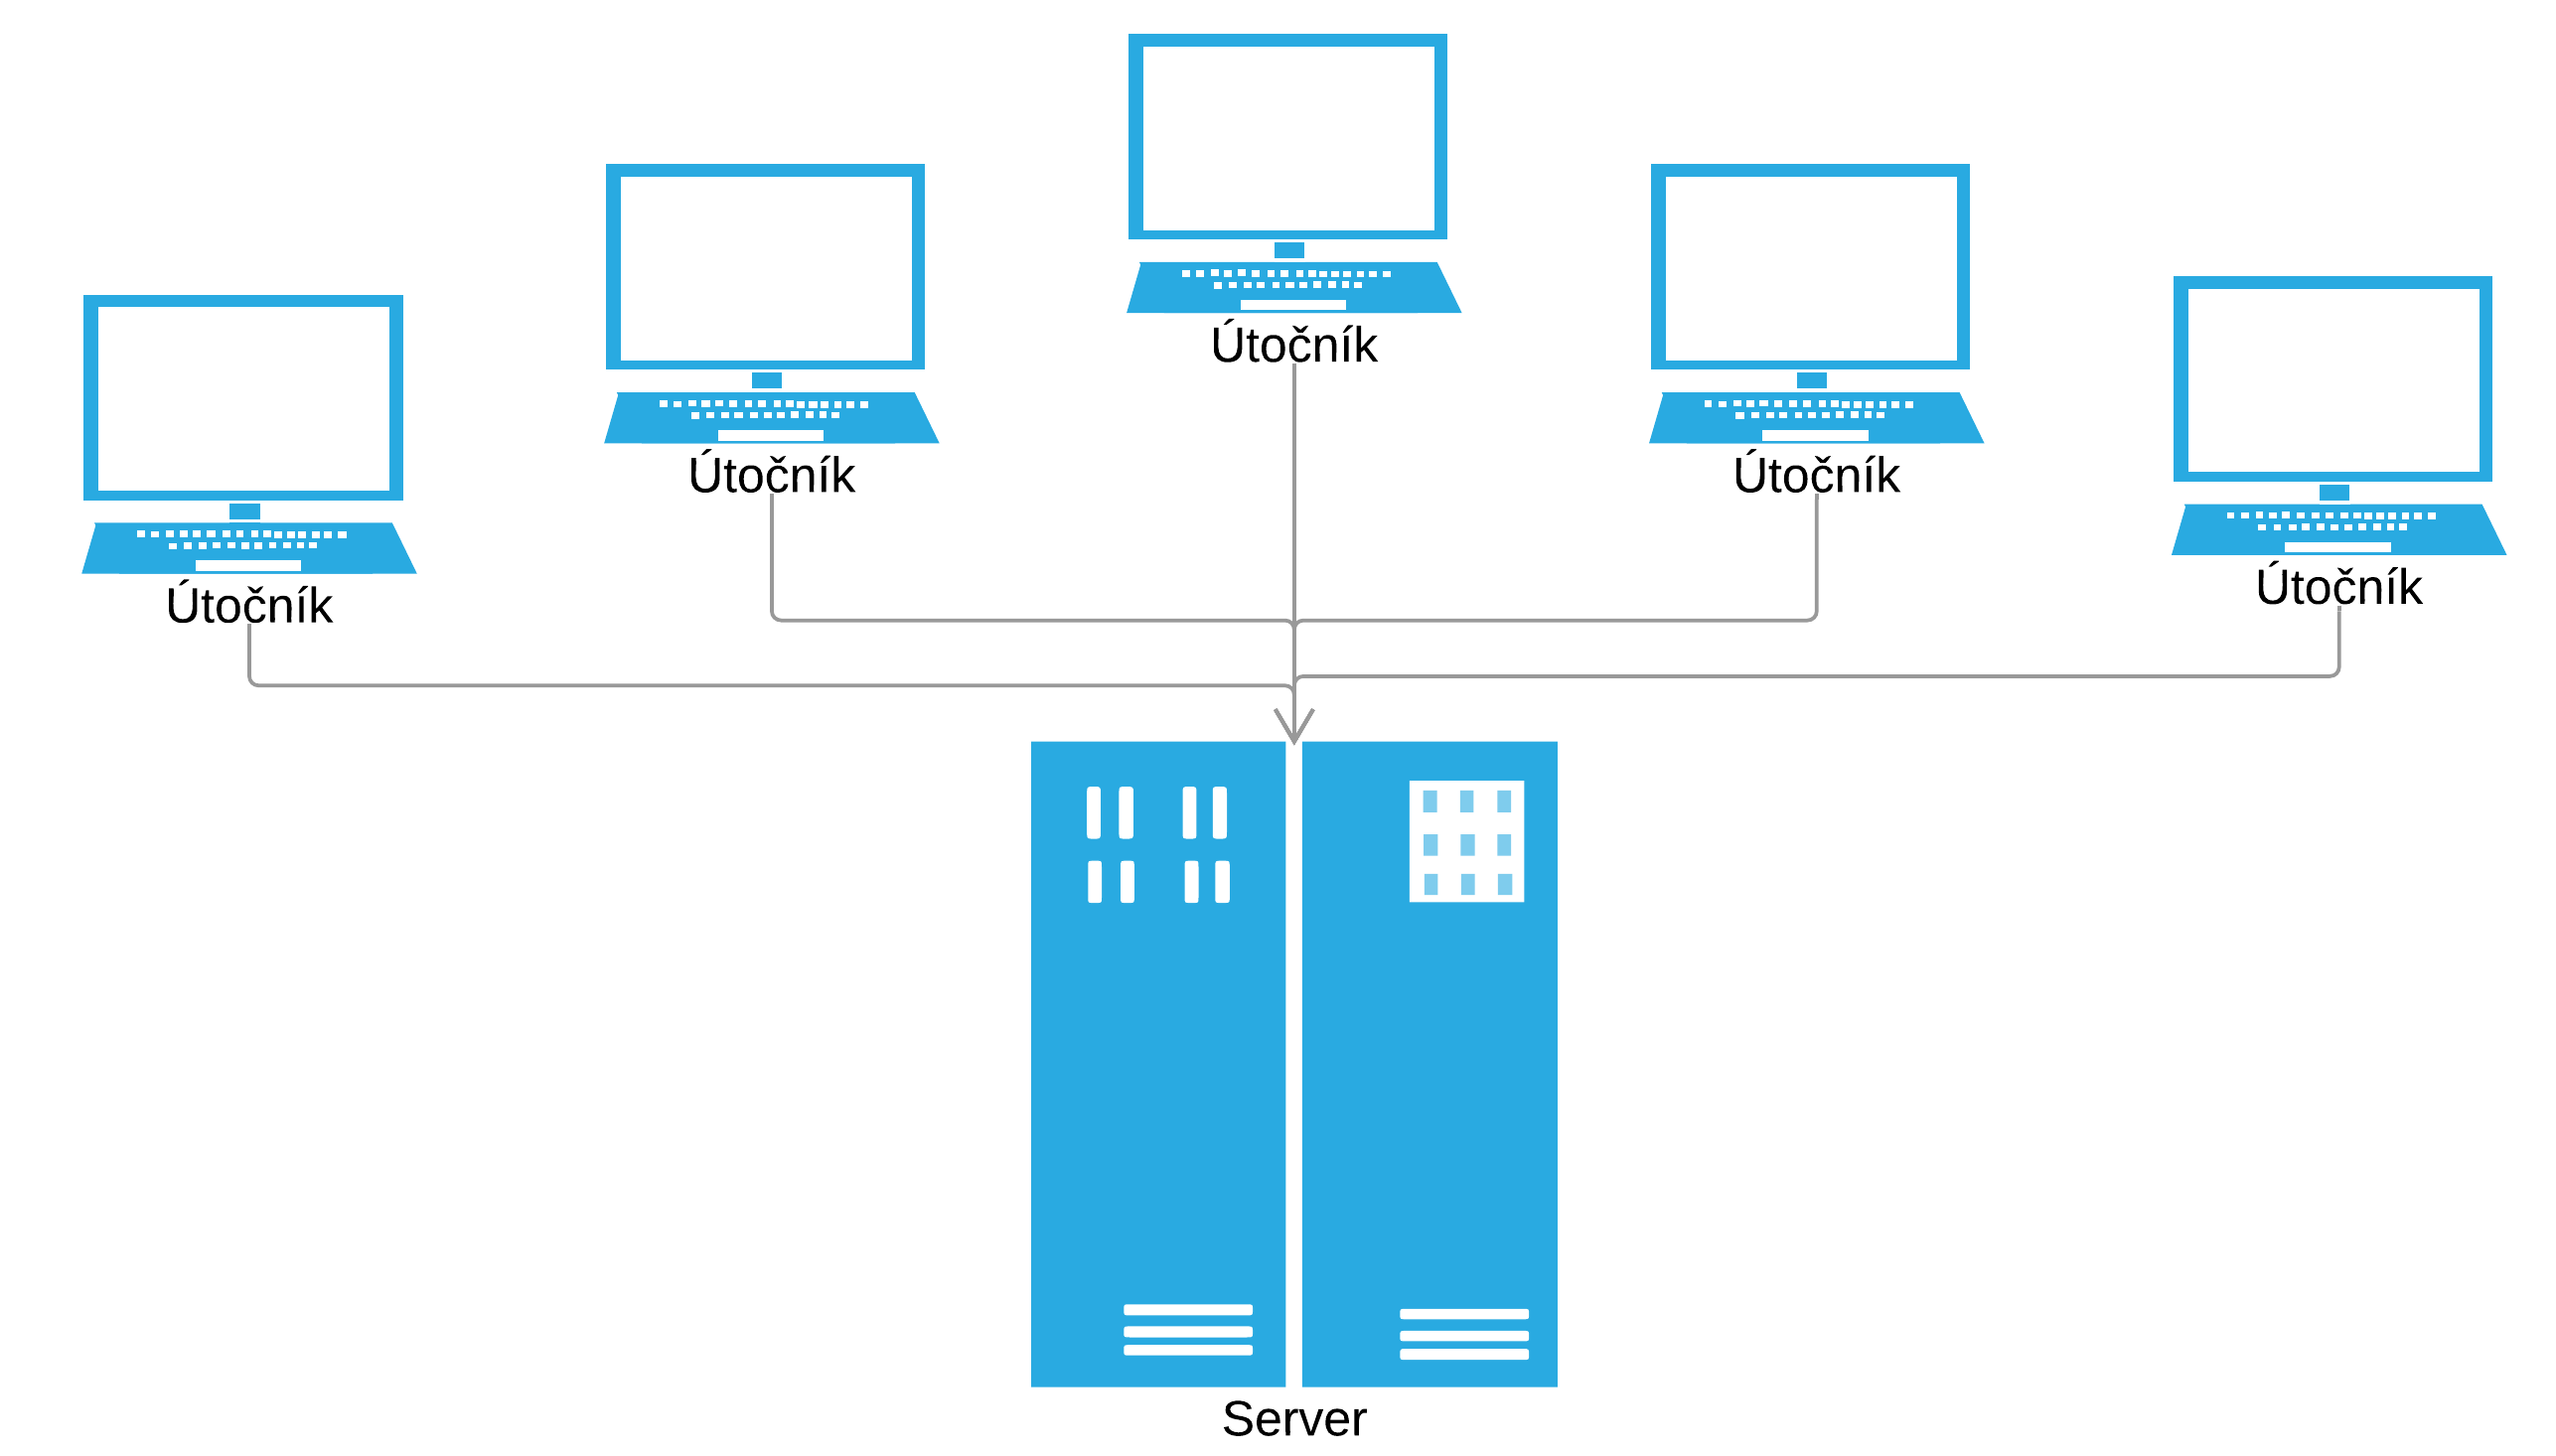
\includegraphics[width=\textwidth]{images/dos.png}
  \caption{Schéma DoS útoku, zdroj: vlastné spracovanie}
  \label{fig:cs-basic}
\end{figure}

U distribuovaného \textit{DoS} útoku môže útočník použiť k útoku na server
počítače klientov. Nad týmito zariadeniami je možné prevziať kontrolu využitím
bezpečnostných chýb alebo nedostatkov. Takto je následne možné donútiť počítač
posielať obrovské množstvo dát na webové servery, prípadne odosielanie nevyžiadanej
pošty na konkrétne e-mailové adresy. Útok sa nazýva "distribuovaný", pretože útočník
používa viac zariadení na začatie útoku \textit{denial-of-service}.

\textit{DoS} útok je podobný veľkej skupine ľudí, ktorá sa zhromažďuje pri vstupe do
obchodu a bráni vo vstupe skutočným zákazníkom, ktorých záujmom sú reálne služby.
Útočníci vykonávajúci tieto útoky sa často zameriavajú na webové služby a servery,
ktoré sú poskytované vysoko profitujúcimi inštitúciami, ako sú napríklad banky,
prípadne platobné brány.

\section{Základne typy a techniky}
Nasledujúce odseky popisujú najpoužívanejšie typy a techniky vykonávania \textit{DoS}
útokov a identifikujú prostriedky, ktorými je im možné zabrániť.

\subsection{Distribuované DoS útoky}
O distribuovaných \textit{DoS} útokoch hovoríme v prípade, že viaceré zariadenia zaplavia
celú šírku pásma prípadne zdrojov cieľového systému, ktorým je zvyčajne jeden, alebo viacero
serverov. Takýto útok je často dôsledkom použitia rôznych systémov a zariadení (napríklad
\textit{botnetu}), ktoré sa snažia vyťažiť cieľový systém. \textit{Botnet} je rozsiahla
virtuálna sieť umelých (\textit{zombie}) počítačov, ktorých cieľom je prijímať príkazy bez
vedomia majiteľa. Keď cieľový systém spotrebuje všetky voľné spojenia, ďalšie (nové) už nie
je možné nadviazať. Hlavné výhody útočníka pri využití Distribuovaného \textit{DoS} útoku
spočívajú v skutočnostiach, že viaceré zariadenia dokážu generovať väčšiu záťaž ako jedno,
pričom použitie množstva systémov zabezpečuje omnoho ťažšiu detekciu útočníka a správanie
sa každého z týchto zariadení je menej pozorovateľné čo sťažuje obranu voči útočníkovi.
Tieto výhody taktiež spôsobujú vývoj obranných mechanizmov. Na strane cieľového serveru už
nebude stačiť jednoduché zvýšenie šírky pásma nad hranicu momentálnej veľkosti útoku, pretože
útočník môže napríklad zvýšiť počet zapojených zariadení čím by taktiež spôsobil zaťaženie a
výpadok systému.

\begin{figure}[H]
  \centering
    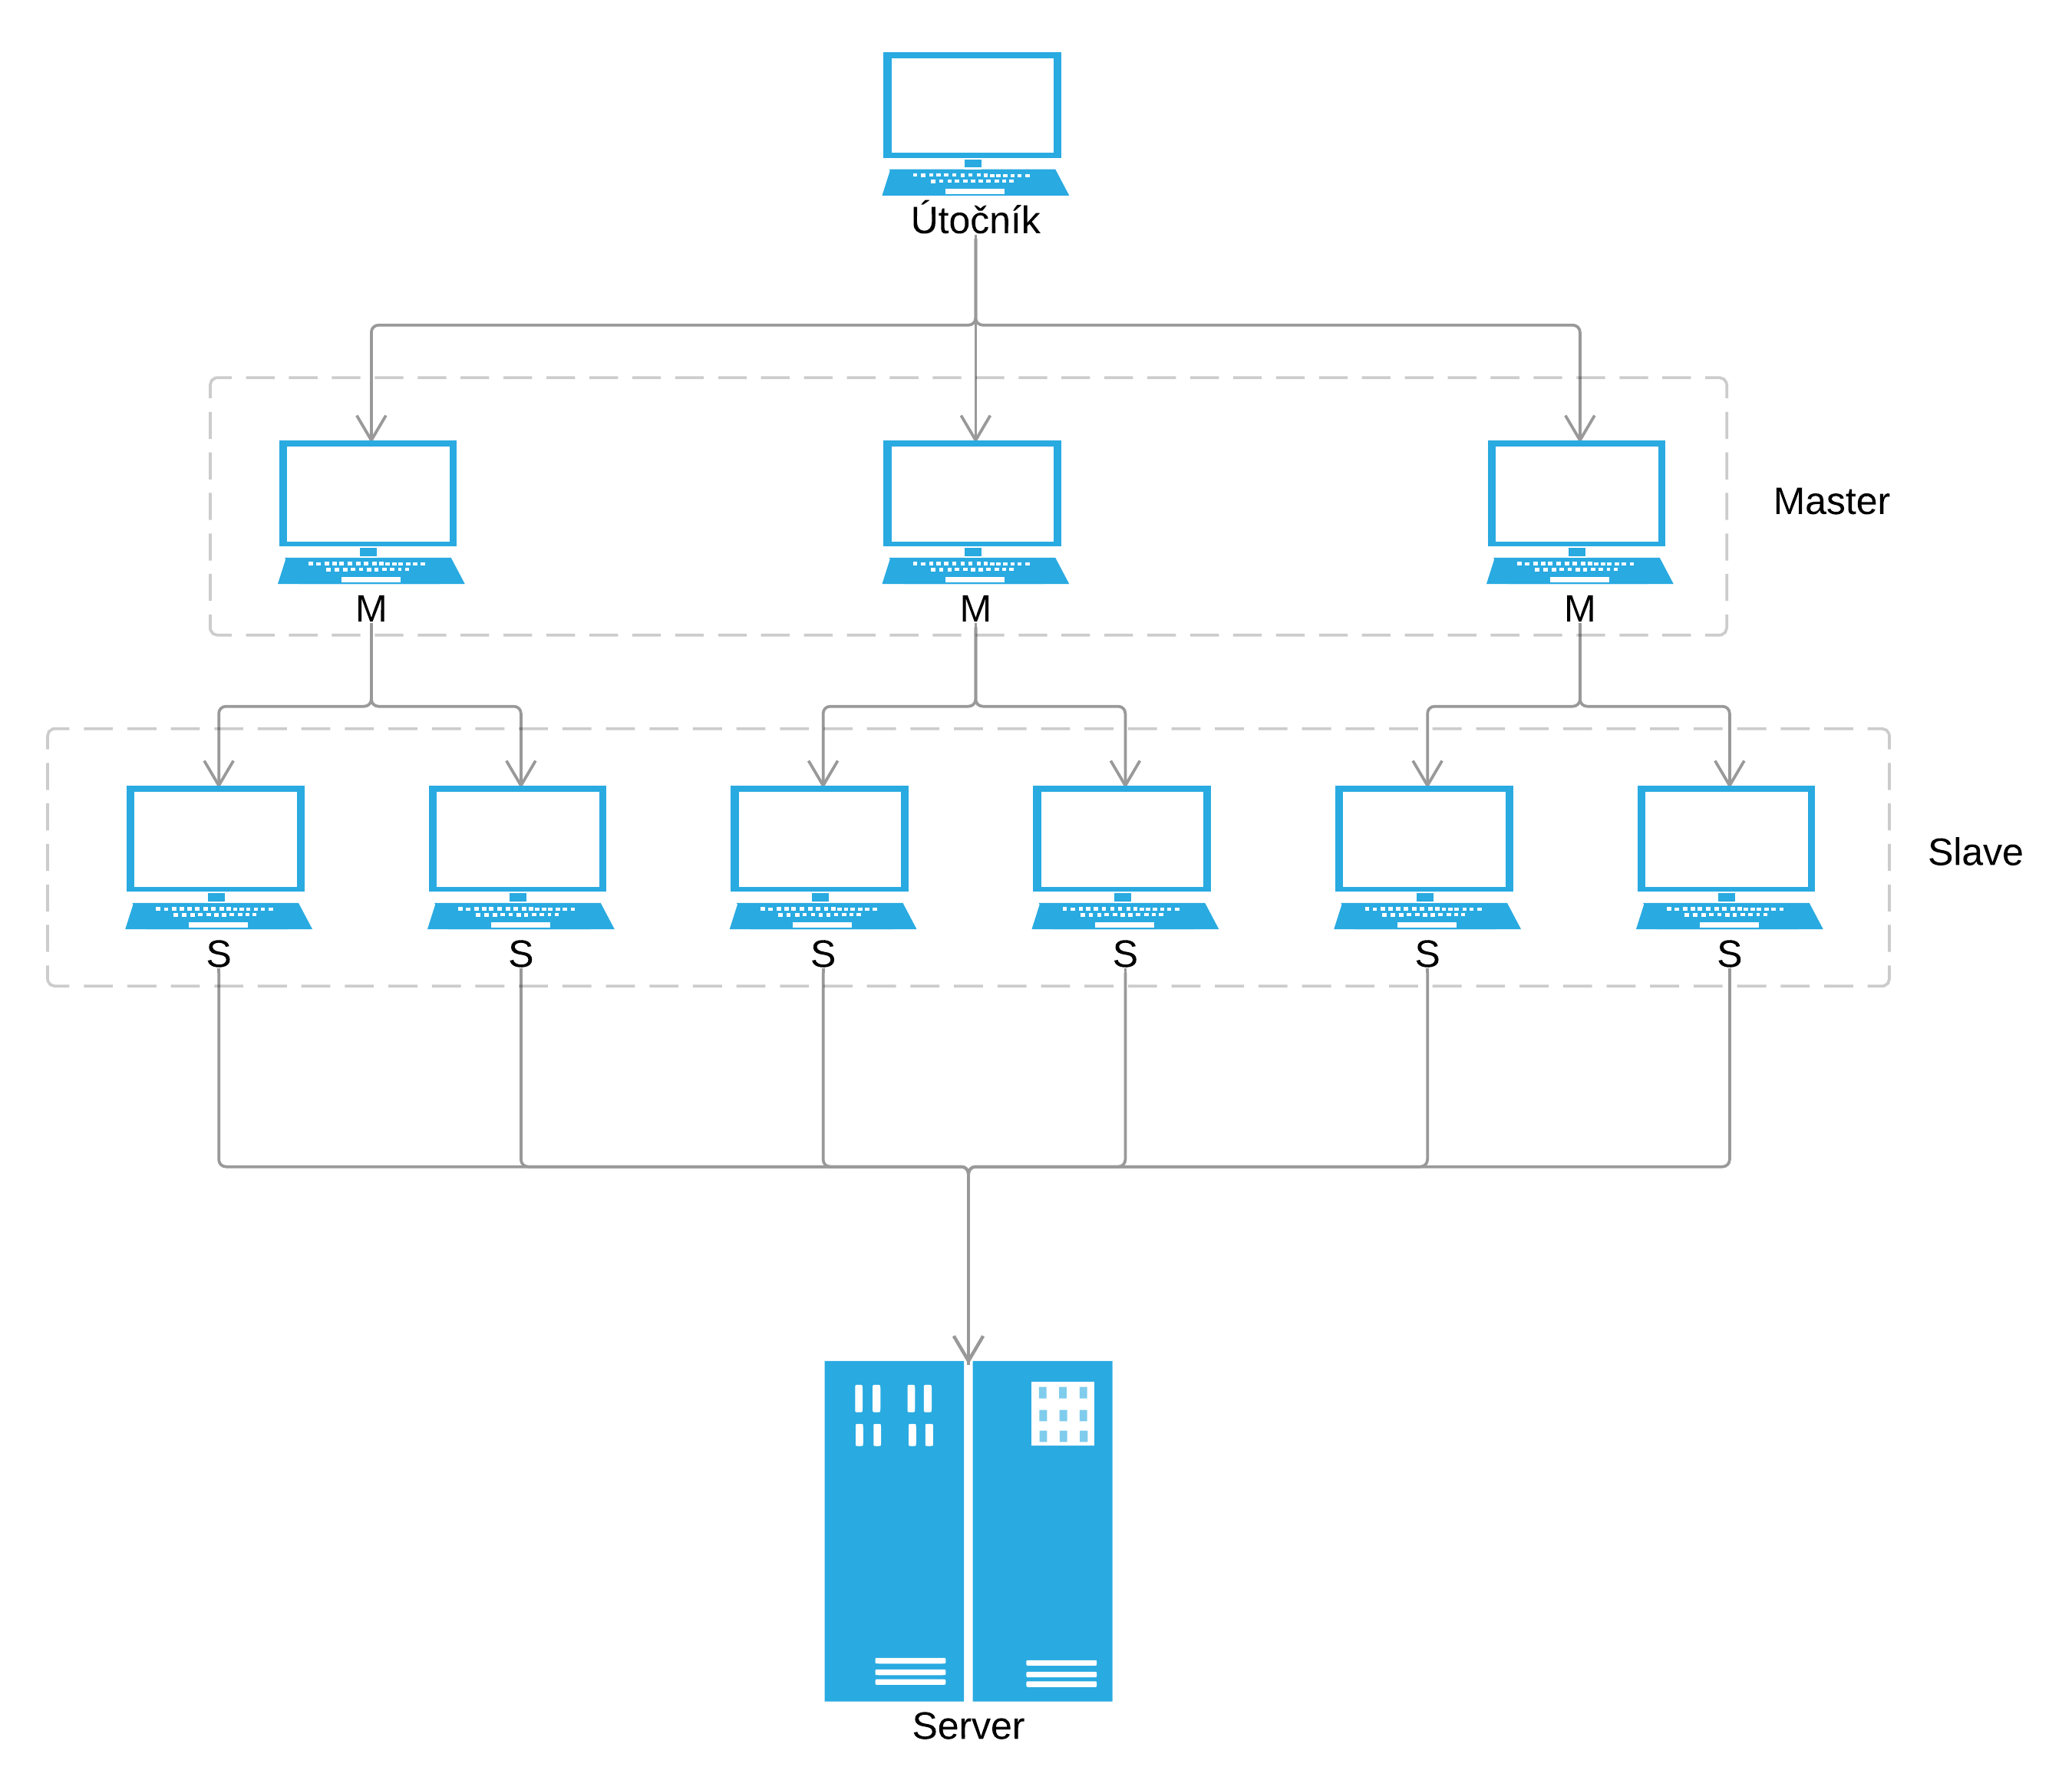
\includegraphics[width=\textwidth]{images/ddos.png}
  \caption{Schéma rozloženia DDoS útoku, zdroj: vlastné spracovanie}
  \label{fig:cs-basic}
\end{figure}

\subsection{Sémantické DoS útoky}
Sémantické útoky využívajú špecifickú funkcionalitu, alebo implementačnú chybu aplikácie,
prípadne protokolu zariadenia obete na zneužitie určitého množstva jeho zdrojov. Napríklad
v prípade \textit{TCP SYN} útoku je touto zneužitou funkcionalitou alokácia značného množstva
priestoru v zozname pripojení ihneď po potvrdení \textit{ TCP SYN requestu}. Útočník otvorí
viaceré spojenia, ktoré nikdy neuzavrie, čím zahlcuje server. 

Pri \textit{CGI} útoku je cieľom útočníka takýmto spôsobom zahltiť procesor viacerými
\textit{CGI requestami}.

Jedným z obzvlášť nebezpečných útokov je \textit{NAPTHA} útok, ktorý sa zameriava na
\textit{TCP} protokol. Inicializuje mnoho \textit{TCP} spojení, ktoré zaplnia zdroje serveru.

\subsection{Brute-force útoky}
TODO 

Source ref: https://www.eecis.udel.edu/~sunshine/publications/ccr.pdf

\subsection{Reflexia a zosilnenie}
TODO
% A reflector is any IP host that will return a packet if sent a packet. Attackers
% orchestrate the hosts under their control to send the spoofed traffic purportedly
% coming from the victim to reflectors. The result is that the flood at the
% victim arrives from a significantly higher number of sources, an exceedingly diffuse
% flood likely clogging every single path to the victim from the rest of the internet.

\begin{figure}[h]
  \centering
    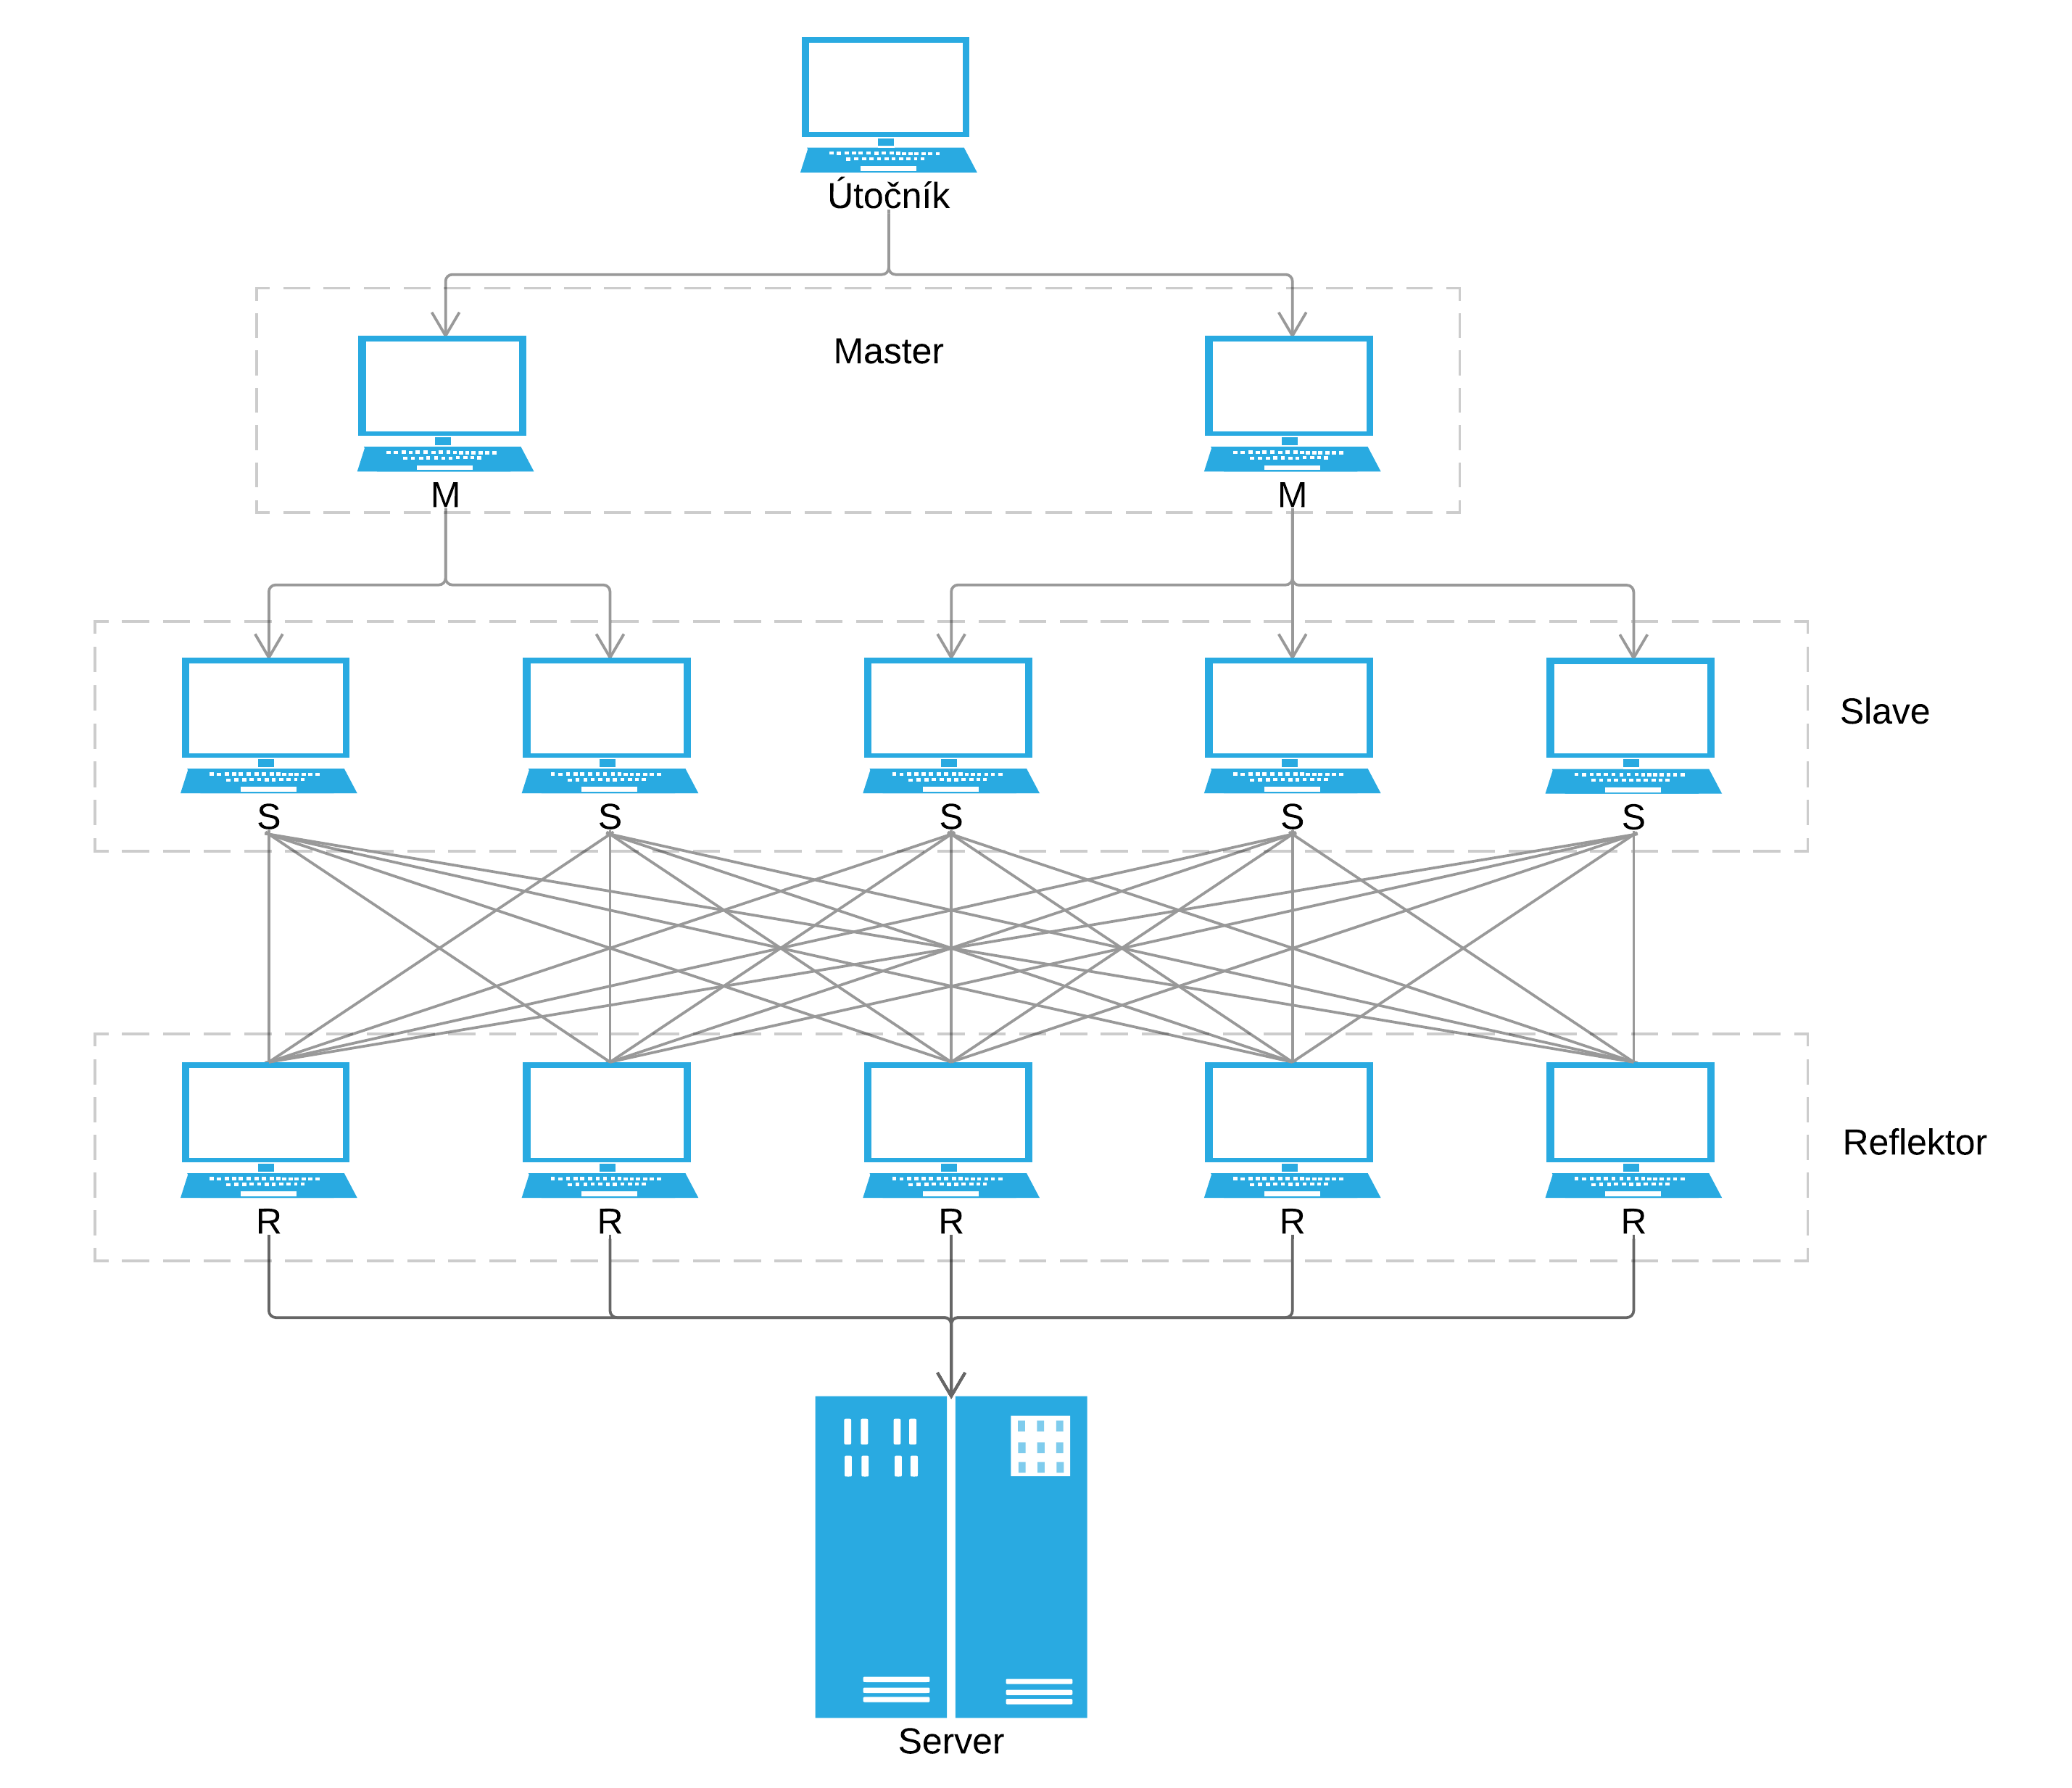
\includegraphics[width=\textwidth]{images/drdos.png}
  \caption{Schéma rozloženia DRDoS útoku, zdroj: vlastné spracovanie}
  \label{fig:cs-basic}
\end{figure}

% Amplification: An amplification attack is a type of the reflection attack in which
% reflectors’ responses are larger than queries. Therefore the volume of the attack
% traffic from the source to the victim is multiplied .

\subsection{HTTP POST DoS útoky}
TODO
% First discovered in 2009, the HTTP POST attack sends a complete, legitimate HTTP POST header, which includes a 'Content-Length' field to specify the size of the message body to follow. However, the attacker then proceeds to send the actual message body at an extremely slow rate (e.g. 1 byte/110 seconds). Due to the entire message being correct and complete, the target server will attempt to obey the 'Content-Length' field in the header, and wait for the entire body of the message to be transmitted, which can take a very long time. The attacker establishes hundreds or even thousands of such connections, until all resources for incoming connections on the server (the victim) are used up, hence making any further (including legitimate) connections impossible until all data has been sent. It is notable that unlike many other (D)DoS attacks, which try to subdue the server by overloading its network or CPU, a HTTP POST attack targets the logical resources of the victim, which means the victim would still have enough network bandwidth and processing power to operate. Further combined with the fact that Apache will, by default, accept requests up to 2GB in size, this attack can be particularly powerful. HTTP POST attacks are difficult to differentiate from legitimate connections, and are therefore able to bypass some protection systems. OWASP, an open source web application security project, has released a testing tool to test the security of servers against this type of attacks.

\section{DoS nástroje a DoS as a Service}
Typickou metódou prenosu mechanizmov \textit{DDoS} útokov je malvér. Jedným z príkladov bol
takzvaný \textit{MyDoom}. Ide o \textit{DoS} mechanizmus, ktorý sa spúšťal vo predom naplánovanom čase.
Tento útok zahŕňal nastavenie hodnoty \textit{IP} adresy cieľového systému pre nasadenie malvéru,
pričom pre spustenie útoku nebola potrebná žiadna interakcia s používateľom.

Ďalším spôsobom zneužitia systému pre \textit{DDoS} útok je použitie skrytej časti softvéru tretej
strany, ktorý umožní útočníkovi stiahnutie \textit{zombie} agenta, prípadne ho už softvér sám obsahuje.
Útočník môže preniknúť do systému taktiež pomocou automatizovaných nástrojov, ktoré zneužívajú chyby v
programoch počúvajúcich vzdialené pripojenia. Tento scenár zasahuje primárne systémy, ktoré sa správajú
ako webové servery. Typickým príkladom \textit{DDoS} nástroja z tejto oblasti je takzvaný
\textit{Stacheldraht}. \textit{Stacheldraht} využíva vrstevnatú štruktúru, v ktorej útočník používa
program klienta na pripojenie sa k \textit{handlerom}, ktoré sú zneužívané na prenos príkazov
k \textit{zombie} agentom. Agenti následne vykonávajú samotný \textit{DDoS} útok. Agenti sú cez handleri
zneužívané útočníkom za pomoci použitia automatizovaných algoritmov na vyhľadávanie zraniteľností v
programoch, ktoré prijímajú vzdialené pripojenia. Každý \textit{handler} je schopný kontrolovať až tisíc
agentov. 

DDoS nástroje ako \textit{Stacheldraht} stále používajú klasické \textit{DoS} metódy zamerané na
zosilnenie a podvrhovanie IP adries ako napríklad útok vyťaženia šírky pásma. Ďalšou z možností je
zahltenie zdrojov - \textit{SYN Flood} útok. Novšie nástroje používajú na \textit{DoS} útoky taktiež
\textit{DNS} servery.

Nástroje ako \textit{MyDoom} môžu byť použité voči ľubovoľnej IP adrese. Menej skúsení útočníci ich
používajú k znemožneniu dostupnosti populárnych a známych webových serverov. Naopak sofistikovanejší
útočníci používajú tieto nástroje na vydieranie, napríklad voči svojim obchodným protivníkom.

V niektorých prípadoch sa však môže zariadenie stať časťou \textit{DDoS} útoku zámerne - so súhlasom
majiteľa. Príkladom je distribuovaný útok \textit{Operation Payback} organizovaný skupinu
\textit{Anonymous}.

---

TODO DoSaaS
% The LOIC has typically been used in this way. Along with HOIC a wide variety of DDoS tools are available today, including paid and free versions, with different features available. There is an underground market for these in hacker related forums and IRC channels.

% UK's GCHQ has tools built for DDoS, named PREDATORS FACE and ROLLING THUNDER.

% Some vendors provide so-called "booter" or "stresser" services, which have simple web-based front ends, and accept payment over the web. Marketed and promoted as stress-testing tools, they can be used to perform unauthorized denial-of-service attacks, and allow technically unsophisticated attackers access to sophisticated attack tools without the need for the attacker to understand their use.

\section{DoS - Zhrnutie}
TODO
% Simple attacks such as SYN floods may appear with a wide range of source IP addresses, giving the appearance of a well distributed DoS. These flood attacks do not require completion of the TCP three way handshake and attempt to exhaust the destination SYN queue or the server bandwidth. Because the source IP addresses can be trivially spoofed, an attack could come from a limited set of sources, or may even originate from a single host. Stack enhancements such as syn cookies may be effective mitigation against SYN queue flooding, however complete bandwidth exhaustion may require involvement.

% If an attacker mounts an attack from a single host it would be classified as a DoS attack. In fact, any attack against availability would be classed as a denial-of-service attack. On the other hand, if an attacker uses many systems to simultaneously launch attacks against a remote host, this would be classified as a DDoS attack.

% It has been reported that there are new attacks from internet of things which have been involved in denial of service attacks. In one noted attack that was made peaked at around 20,000 requests per second which came from around 900 CCTV cameras.


\chapter{Existujúce prístupy k identifikácií}
\label{ch:existing}
Nasledujúca kapitola sa venuje popisu, porovnaniu a hodnoteniu existujúcich
prístupov, ktoré sú momentálne využívané na účely identifikácie používateľa.
Ide najmä o techniky využívajúce: protokoly sieťovej vrstvy (najmä IP adresy),
monitorovanie TCP komunikácie a vlastné aplikačné identifikátory.

\section{Využitie sieťovej vrstvy}
Jedným z najtypickejších spôsobov identifickácie užívateľa a jeho zriadenia je
IP protokol sieťovej vrstvy. Táto technika je veľmi rozšírená napíklad pre
účely blokovania prístupu na server u systémových \textit{firewallov} a
podobne.

\subsection{Internet Protocol (IP)}
Ako popisuje kapitola \ref{ch:net-layers} Internet Protocol slúži na prenos paketov
medzi jednotlivými sieťovými uzlami - zariadeniami, ktoré sú identifikovné
IP adresami. V ideálnom 


\subsection{Vyhody a nevyhody}
\section{Monitoring TCP}
//TODO - Popis
\subsection{Vyhody a nevyhody}
\section{Aplikačné identifikátory}
//TODO - Popis
\subsection{Vyhody a nevyhody}
\section{Zhrnutie}

\chapter{Tvorba unikátneho identifikátoru}
\label{ch:footprint}
//TODO - Úvod
\section{Možnosti protokolu HTTP}
\section{Možnosti TCP}
\section{Popis Algoritmu}

\section{Záver}

\makeatletter\thesis@blocks@clear\makeatother
\phantomsection %% Print the index and insert it into the
\addcontentsline{toc}{chapter}{\indexname} %% table of contents.
\printindex

\appendix %% Start the appendices.
\chapter{Príloha}
Appendices of thesis.

\end{document}
